\chapter{OpenGL/3D Workflow}
\label{cha:ogl}
\minitoc

Aufgrund der komplexen Struktur bei der Konfiguration des 3D
Subsystems unter Linux, wird dieser Teil hier gesondert dokumentiert.
Zur Konfiguration sind folgende Dinge zu beachten:

\begin{enumerate}
\item Pr"ufen und installieren der notwendigen 3D Pakete falls noch
      nicht geschehen. Es gibt unter Linux einige Ans"atze um die 3D
      Unterst"utzung zu realisieren. Leider hat sich dabei noch kein
      Standard herausgebildet und aus diesem Grund gibt es viele
      verschiedene Pakete von denen ganz bestimmte f"ur eine
      bestimmte Klasse von Karten notwendig sind. \textbf{xapi} 
      "ubernimmt diese Aufgabe im Bedarfsfall mit Hilfe von YaST2 oder
     dem YaST2 Online-Update.  
\item Erkennen und einstellen aller notwendigen Konfigurationsparameter.
      Dies betrifft haupts"achlich die Wahl der passenden 3D Module und
      des Treibers der die Karte 3D m"a"sig unterst"utzt. 
\end{enumerate}

\section{3D Schema}
Dreh und Angelpunkt ist auch in diesem Fall die
\textbf{Identity.map} Datei. Sie enth"alt ein Verzeichnis aller
uns bekannten und unterst"utzten Karten. Die Erkennung einer 3D
Karte funktioniert nach folgendem Schema:
\begin{enumerate}
\item Durch die SaX2 Initialisierung via \textit{init.pl} wird
      unter anderem der sysp Aufruf zur Ermittlung
      von Serverdaten (sysp -s server). Hier wird der PCI/AGP Bus
      ausgelesen und die Karte identifiziert. Stellt sysp fest, da"s
      die erkannte Karte auch im 3D Bereich arbeiten kann so wird
      eine Frage an den Benutzer gestellt ob er die Karte im 3D
      Bereich betreiben will. Dies setzt zwei Identity Eintr"age
      f"ur ein und dieselbe Karte voraus:
      \begin{itemize}
      \item Der 2D Eintrag erh"alt das FLAG=DEFAULT
      \item Der 3D Eintrag erh"alt das FLAG=3D
      \end{itemize}
      Damit ist die Karte eindeutig spezifiziert und es steht
      zu diesem Zeitpunkt schon fest:
      \begin{itemize}
      \item Welcher Treiber verwendet werden muss
      \item Welche Optionen notwendig sind
      \item Welche Extensions einzuschalten sind (Module)
      \item Welches Profil notwendig ist
      \item Welche Pakete gebraucht werden
      \item Welches 3D Script aufgerufen werden muss
      \end{itemize}
\item Im weiteren Verlauf der Initialisierung wird ein weiteres
      sysp Modul aufgerufen: \textbf{Scan3Dlib.pm} Dieses Modul
      verarbeitet die Paketdaten und installiert/updated die 
      erforderlichen Pakete, entscheidet welches 3D Script aufzurufen ist
      und speichert den aktuelle Zustand des 3D Subsystems.
      Die 3D-Skripte sind in den jeweiligen 3D Paketen 
      enthalten.
\item Stellt \textbf{init.pl} fest, da"s es sich um eine erst-Initialisierung
      handelt oder die Hardware ge"andert wurde, dann wird das 3D Skript
      an dieser Stelle aufgerufen. Welches Skript das ist, h"angt von
      dem Eintrag in der Identity.map und von der Antwort auf die 3D Frage
      ab. 
      \begin{itemize}
      \item Mit dem Abschlu"s der Initialisierung erfolgt die zweite
            Stufe der Konfiguration \textbf{(xapi)}. Hier ist es wichtig zu
            wissen, da"s die "Uberpr"fung der Paketinformationen aus 
            Scan3Dlib nur innerhalb von \textbf{xapi} passiert und damit
            bei einer vollst"andig automatischen Konfiguration "uber den
            Parameter \textit{--auto} nicht ausgef"uhrt wird.
            In diesem Fall wird zwar eine 3D Konfiguration geschrieben aber
            es kann sein, da"s die notwendigen Pakete nicht vorhanden sind.
      \end{itemize}
      Das folgende Schaubild zeigt den Ablauf des 3D Schemas
      Es stellt nur den Teil des Gesammtworkflows dar, der f"ur die 3D
      Einrichtung wichtig ist.

      \index{Schaubild 3D}
      \begin{figure}[h]
      \centering
      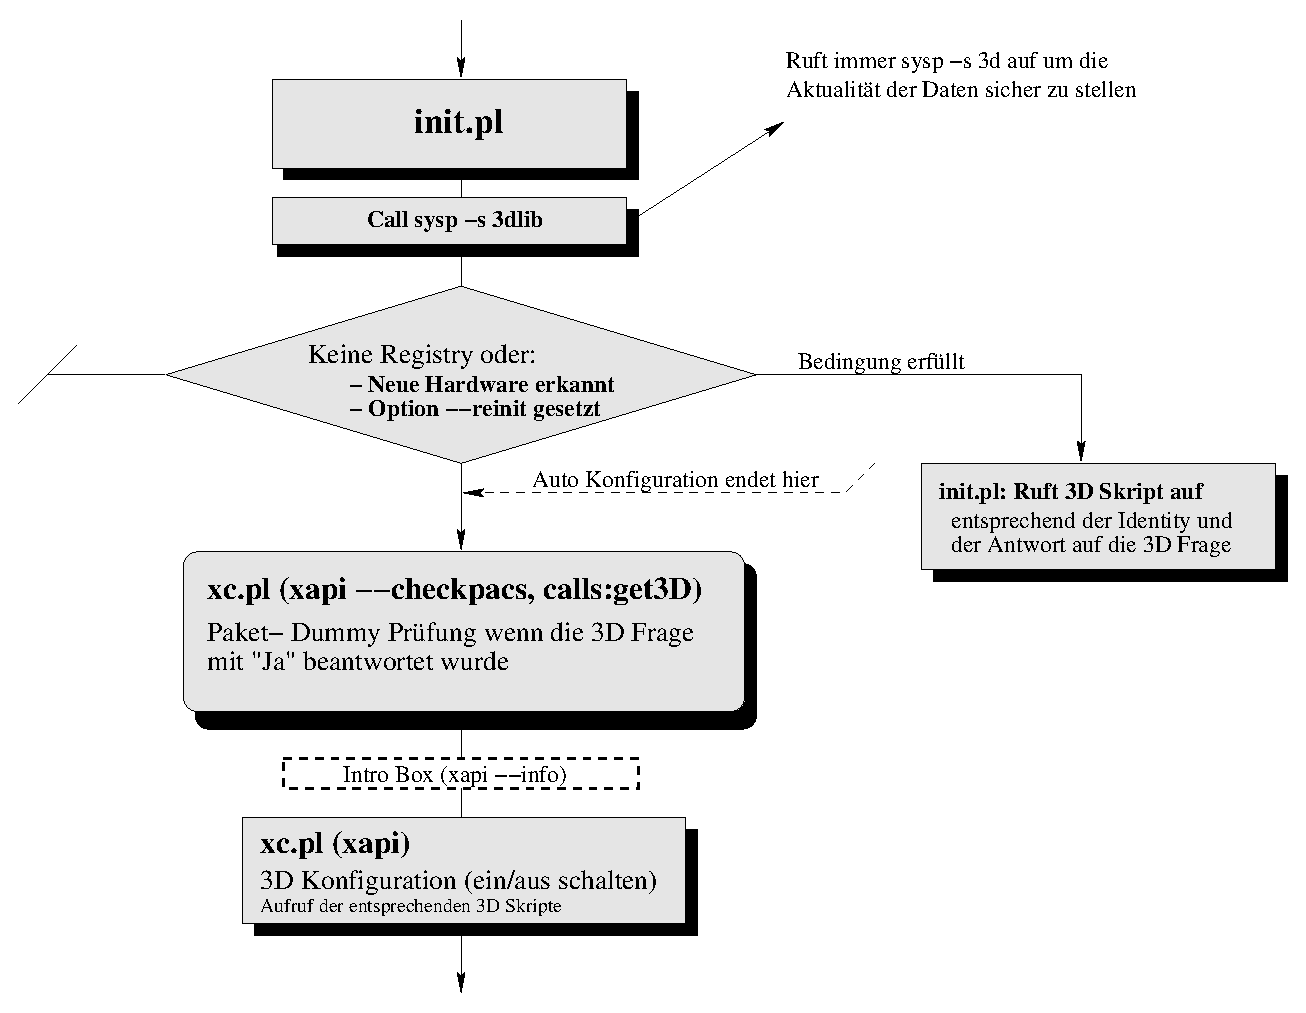
\epsfig{file=pictures/3d.ps,width=10cm}
      \caption{Flussdiagramm SaX2 (3D Teil)}
      \end{figure}

\item In der zweiten Stufe der Konfiguration (xapi) wird der aktuelle
      Zustand des 3D Subsystems "uber das \textbf{get3D} Skript abgefragt
      und verarbeitet. Die 3D Konfiguration kann nun "uber den 3D/OpenGL
      Dialog ein- bzw. Ausgeschalten werden. Die folgende Liste zeigt,
      den Ablauf beim ein- bzw Ausschalten der 3D Umgebung:
      \begin{itemize}
      \item \textbf{3D Ausschalten...}
            \begin{enumerate}
            \item Aufruf des \textbf{switch2mesasoft} 3D Skripts
            \end{enumerate}
      \item \textbf{3D Einschalten...}
            \begin{enumerate}
            \item Hinzuf"ugen der 3D extension Module
            \item Farbtiefe auf 16Bit pr"ufen und eventuell eine
                  Warnung ausgeben
            \item 3D Pakete entsprechend der selektierten Karte
                  pr�fen. Ausgabe einer Warnung falls nicht installiert
            \item 3D NVidia dummy Treiber pr�fen. Ausgabe einer
                  Warnung falls online Update notwendig
            \item Aufruf des 3D Skripts
            \end{enumerate}
      \end{itemize}
      Die Informationen bez"uglich Treiber, Optionen, Extensions, etc.
      entstammen hierbei den CDB Daten welche ein Abbild der 
      \textit{Identity.map} sind. Es ist daher immer notwendig, da"s
      die entsprechende Karte in der Liste der Graphikkarten vorhanden
      und selektiert ist.
\end{enumerate}
